\documentclass[11pt,a4paper]{article}
\usepackage{geometry}
\geometry{letterpaper, portrait, left=1in, right=1in, top=1in, bottom=1in}
\usepackage[utf8]{inputenc}
\usepackage{amsmath}
\usepackage{amsfonts}
\usepackage{amssymb}
\usepackage{multicol}
\usepackage{enumitem}
\usepackage{lipsum}
\usepackage[final]{graphicx}
\DeclareGraphicsExtensions{.pdf,.png,.jpg}
\usepackage[english]{babel}
\usepackage{csquotes}
\usepackage[backend=bibtex]{biblatex}
\bibliography{mybib}
\usepackage{hyperref}
\hypersetup{
	linktoc=all,
	filecolor=magenta,      
	urlcolor=cyan,
	bookmarks=true  
}

\begin{document}
	\title{Project Report - Team N64}
	\author{Neil Ryan, Steven Kool, Rachel Yanovsky}
	\maketitle
	\newpage
	\tableofcontents
	\newpage
	
	\section{Statement of Use}
	We grant permission to any person to use any part of this project under the "Beerware" license, detailed below:\\\\
	\textbf{This project was written by Rachel Yanovsky, Steven Kool, and Neil Ryan.\\As long as you retain this notice you
	can do whatever you want with this stuff. \\
	If we meet some day, and you think this stuff is worth it, you can buy us a beer in return.} \\
	
	
	Our project can be found at the following link:\\
	\url{https://github.com/soctar/GBA}\\\\
	
	Feel free to contact us with any questions:\\
	\href{mailto:nryan@andrew.cmu.edu}{nryan@andrew.cmu.edu}\\
	\href{mailto:skool@andrew.cmu.edu}{skool@andrew.cmu.edu}\\
	\href{mailto:ryanovsk@andrew.cmu.edu}{ryanovsk@andrew.cmu.edu}\\
	\newpage
	\section{Origin of the Team Name}
	Originally, we were floating the idea of extending the N64 project from 2014 instead of a GameBoy Advance. The N64 project had a mostly working CPU, the main work would be the Reality Co-Processor (RCP), which is the main DSP and GPU for the Nintendo 64. The pipeline of the N64 is such that everything flows through this chip, and the documentation for the RCP is fairly sparse. From the previous N64 group's report, we found \href{https://github.com/tj90241/cen64}{cen64}, a cycle accurate N64 emulator that currently runs Super Mario 64 and a host of other games with high accuracy.\\\\
	The Reality Co-Processor is made up of two chips, the Reality Signal Processor (RSP) and Reality Display Processor (RDP). We reached out to Tyler Stachecki, the creator of cen64, to see if he had some sort of emulator for just the RCP, or preferably emulators for the RSP and RDP. For posterity, we've included his response below, with important sections in bold. If future students ignore all of our advice at least heed this: Do not attempt an N64. It is a wholly unreasonable project for a semester. Perhaps if several groups dedicated themselves to sections of it, it might be only a stretch, but even with 8 highly talented engineers, we feel as though the project would be doomed to fail.\\\\
	\\
	Hi Neil,\\\\
	I still remember working with last years' folks! Very neat to see this
	project being continued and wish you the best of luck.\\\\
	The RCP is not completely cycle-accurate yet by any means. CEN64's
	implementation of the RSP (the vector processor within the RCP, used
	for both audio mixing and T\&L) is written in a quasi cycle-accurate
	manner [1], as was the VR4300 that last years' students worked on.
	Probably the biggest difference between the RSP model that I've
	written and hardware is that the latter will dual-issue instructions
	under certain conditions, while my pipeline unconditionally
	single-issues for the time being. I've got the backend logic ready for
	dual-issue (you will see that rsp\_cycle\_ invokes both rsp\_v\_ex\_cycle
	and rsp\_ex\_cycle), but the frontend is still dual-issue agnostic.\\\\
	Also regarding the inaccuracy of the RSP, there are also some timing
	differences -- e.g.., CEN64 doesn't simulate the DMAs, it just
	completes the command in a single cycle. The other components of the
	RCP (the audio, cart, controller, etc.) blocks are written in a
	similar manner in that they either use fixed time-delay models or also
	just complete commands in a single cycle. However, this is something
	you can easily work around in HDL since everything is interrupt-driven
	-- notice that virtually everything controller or CPU in the console
	will atomically set local MMIO registers and raise an interrupt when
	they're done with their DMA operation or whatever else.\\\\
	The RDP, on the other hand, is considerably more difficult for the
	following reasons:
	\textbf{1) There only exists one open-source software (pixel-accurate)
	renderer which all current N64 emulators share (which was originally
	derived from MAME). I encourage you to look at it, because the coding
	style used is absolutely horrendous and very well may be the most vile
	thing you've ever laid eyes on. Trying to digest everything that the
	RDP is doing, nevermind writing a simulator or HDL, will be quite a
	bit of work in and of itself.}\\\\
	2) The RDP does *not* raster triangles in a manner similar to
	virtually any other piece of graphics hardware. Read this forum post
	[2] as it's a really good summary of how the RDP renders things.\\\\
	3) Also keep in mind that the N64 uses a unified memory model - not a
	single CPU has any memory that is dedicated to it (aside from it's
	caches) -- so you would need to arbitrate accesses and get all the
	timing sorted out for this as well. Since you're working on the clock
	speeds of an FPGA, SDRAM definitely won't cut it and you'll probably
	find that you need to use (at least) DDR2 for the bandwidth you're
	looking for. The RDRAM in the N64 is clocked at 250MHz and operates on
	both edges of the clock (and since it's RDRAM, the data bus is 9 bits
	wide -- not 8 bits!) The RDP actually uses the 9th bit for coverage
	information, so you can't ignore that fact and you'd likely have to
	drive two ranks of memory in parallel. You could also just use
	blockram on the FPGA, but I'm not sure you'll have access to something
	with enough blockram available.\\\\
	tl;dr: My advice to you would be the same as the last years' team and
	was reflected in their report - do NOT bite off more than you can
	chew. I don't think it's possible to 'clone' the RCP in one semester,
	even with a team of 3-4 very talented and dedicated engineers. If you
	want to do something graphics-oriented, I would ignore the entirety of
	the RCP and only try to write HDL for the RDP (and that in and of
	itself is quite a bit of work, for the reasons mentioned above). You
	can use last year's work to "drive" the RDP -- have it write the
	display lists to memory and treat the RDP as an interrupt-driven
	signal processor (the console effectively does the same thing). If you
	hack a little bit on CEN64, you should be able to get it it to dump
	the display lists (the "instructions") that real game carts are
	ultimately sending to the RDP, along with all the texture data and
	whatnot. In theory, you can just "play back" these display lists to
	the RDP to get it to render realtime content for your demo at the end
	of the semester demo. FYI: I'd first investigate the size and
	bandwidth required for these display lists -- double check to make
	sure it's something that's feasible with what your FPGA provides.\\\\
	
	Let me know what you end up doing!\\
	Tyler\\\\
	
	[1] \url{https://github.com/tj90241/cen64/blob/master/rsp/pipeline.c\#L208}\\
	
	[2] \url{http://forums.cen64.com/viewtopic.php?f=14\&t=237}
	
	
	\newpage
	\section{Overview}
	The GameBoy Advance (GBA) was an extremely popular handheld console by Nintendo, released in 2001, succeeding the GameBoy Color. As with previous Nintendo handheld consoles, it was a single-player device, with the option of attaching a link cable between devices for multiplayer interactions. The serial port on the top of the device that the link cable attached to was also used for a wireless adapter in \textit{Pokemon: Fire Red and Leaf Green}, as well as for links between the Nintendo GameCube and the GameBoy Advance. The GameBoy Advance was also backwards compatible with GameBoy Color games.\\\\
	The Game Boy Advance (GBA) is composed of four major subsystems - the ARM7TDMI CPU, the graphics pipeline, the sound engine, and the Link Cable serial interface. The GBA also includes a Zilog Z80 processor for backwards GameBoy Color compatibility. Additionally, the Game Boy Advance contains a Direct Memory Access (DMA) controller, several programmable timers, an interrupt controller, and 10 buttons. The graphics pipeline outputs to a 240x160 RGB LCD screen; the sound outputs to either a mono speaker, or the GBA's stereo headphone jack. The system clock is the same as the CPU clock, running at 16.78MHz.\cite{GBAManual} \\\\	
	On a high level, the GBA architecture is a MMIO register based system. The ARM7TDMI acts as a master to configure the various subsystems. Generally, registers act as control points, but are occasionally used to give the status of subsystems to the CPU.\\\\
	Initially, we had planned to finish the semester with a working GameBoy Advance that could play three games: Pokemon Ruby, Legend of Zelda: Minish Cap, and Kim Possible 3: Team Possible (the favorite childhood games of our group members), but several aspects of the project ended up taking much, much longer than we anticipated. We feel, however, that enough dense roadblocks have been dealt with to make this a very achievable project for future groups to complete.
	
	\subsection{GBA Architecture}
	While the GBA generally operates in a master-slave fashion, there are several points of interactions between the subsystems. For the most part in this project, we made no attempt to create a cycle accurate system. It is possible that some games exist that abuse the specifics of the hardware enough to make this a problem, but from our understanding of the GBA specification, there is little incentive to cut game timing close enough to make this a problem - the "hacky" characteristics of some 80s arcade cabinets are unlikely to be present in the GameBoy Advance. Namely, games are likely compiled, instead of hand-assembled.\\\\
	As previously stated, the ARM7TDMI core controls most of the system. The GBA only has one memory bus which is shared by all subsystems. To avoid multiple drivers, DMA takes priority over the CPU and pauses the CPU when it is active. Additionally, the CPU and DMA cannot read from graphics memory outside of VBLANK and HBLANK. While not in a display blanking period, the graphics has control over the memory ports to the three sections of VRAM, OAM, and Palette RAM. \\\\
	
	\subsection{GBA Schematic}
	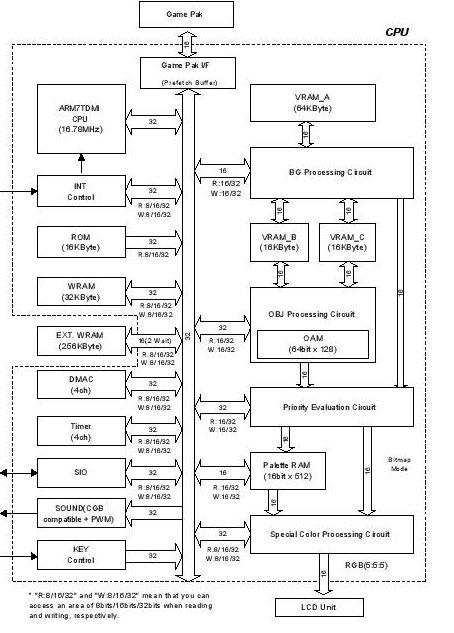
\includegraphics[width=12cm, height=18cm, keepaspectratio=true]{gbaschematic}
	
	
	\subsection{System Diagram}
	\includegraphics[width=12cm, height=8cm, keepaspectratio=true]{system}
	
	\section{Infrastructure}
	\subsection{Custom ROMs}
	A healthy amount of googling can get pretty much any ROM for the GameBoyAdvance, but it can be extremely helpful to be able to write custom ROMs for testing (or if a final demo needs to be scaled back). Conveniently, a surprisingly large group of hobbyists find programming games for the GBA to be enthralling. We used the DevKitARM toolchain - a tutorial is at the link below.\\
	
	\url{https://www.reinterpretcast.com/writing-a-game-boy-advance-game}
	 
	\subsection{Emulators}
	Many emulators exist for the GameBoy Advance - none claim to be cycle accurate (that we found that worked). For debugging, we primarily used mGBA and no\$gba - specifically the "full" version of no\$gba. In most cases, no\$gba was more valuable, but mGBA gives the current state of memory - no\$gba only gives the state of memory at boot (only memory locations defined by the BIOS and the GamePak are valid).\\\\
	No\$gba (pronounced No-cash-gba), however, has some poorly documented behavior. First, to boot the BIOS in No\$gba, there needs to be a BIOS file in the same directory as \texttt{NO\$GBA.exe} named \texttt{gba.rom}. Second, breakpoints are set in a format completely unique to no\$gba - for example, to break on any writes to addresses between \texttt{0x040000A0} and \texttt{0x040000A4} (DMA FIFO), the format is \texttt{[040000A0..040000A4]!!}. More details are in the breakpoints help dialog in no\$gba.\\
	In the strange and bizarre case that future groups fail to realize exactly how powerful no\$gba, a screenshot of BIOS debugging is below. A zip archive of no\$gba is in our Git repository which includes everything needed to run the debugging version except ROMs (which should be stored in the SLOT folder) and the BIOS (which should be stored in the top level folder, named \texttt{gba.rom}).\\
	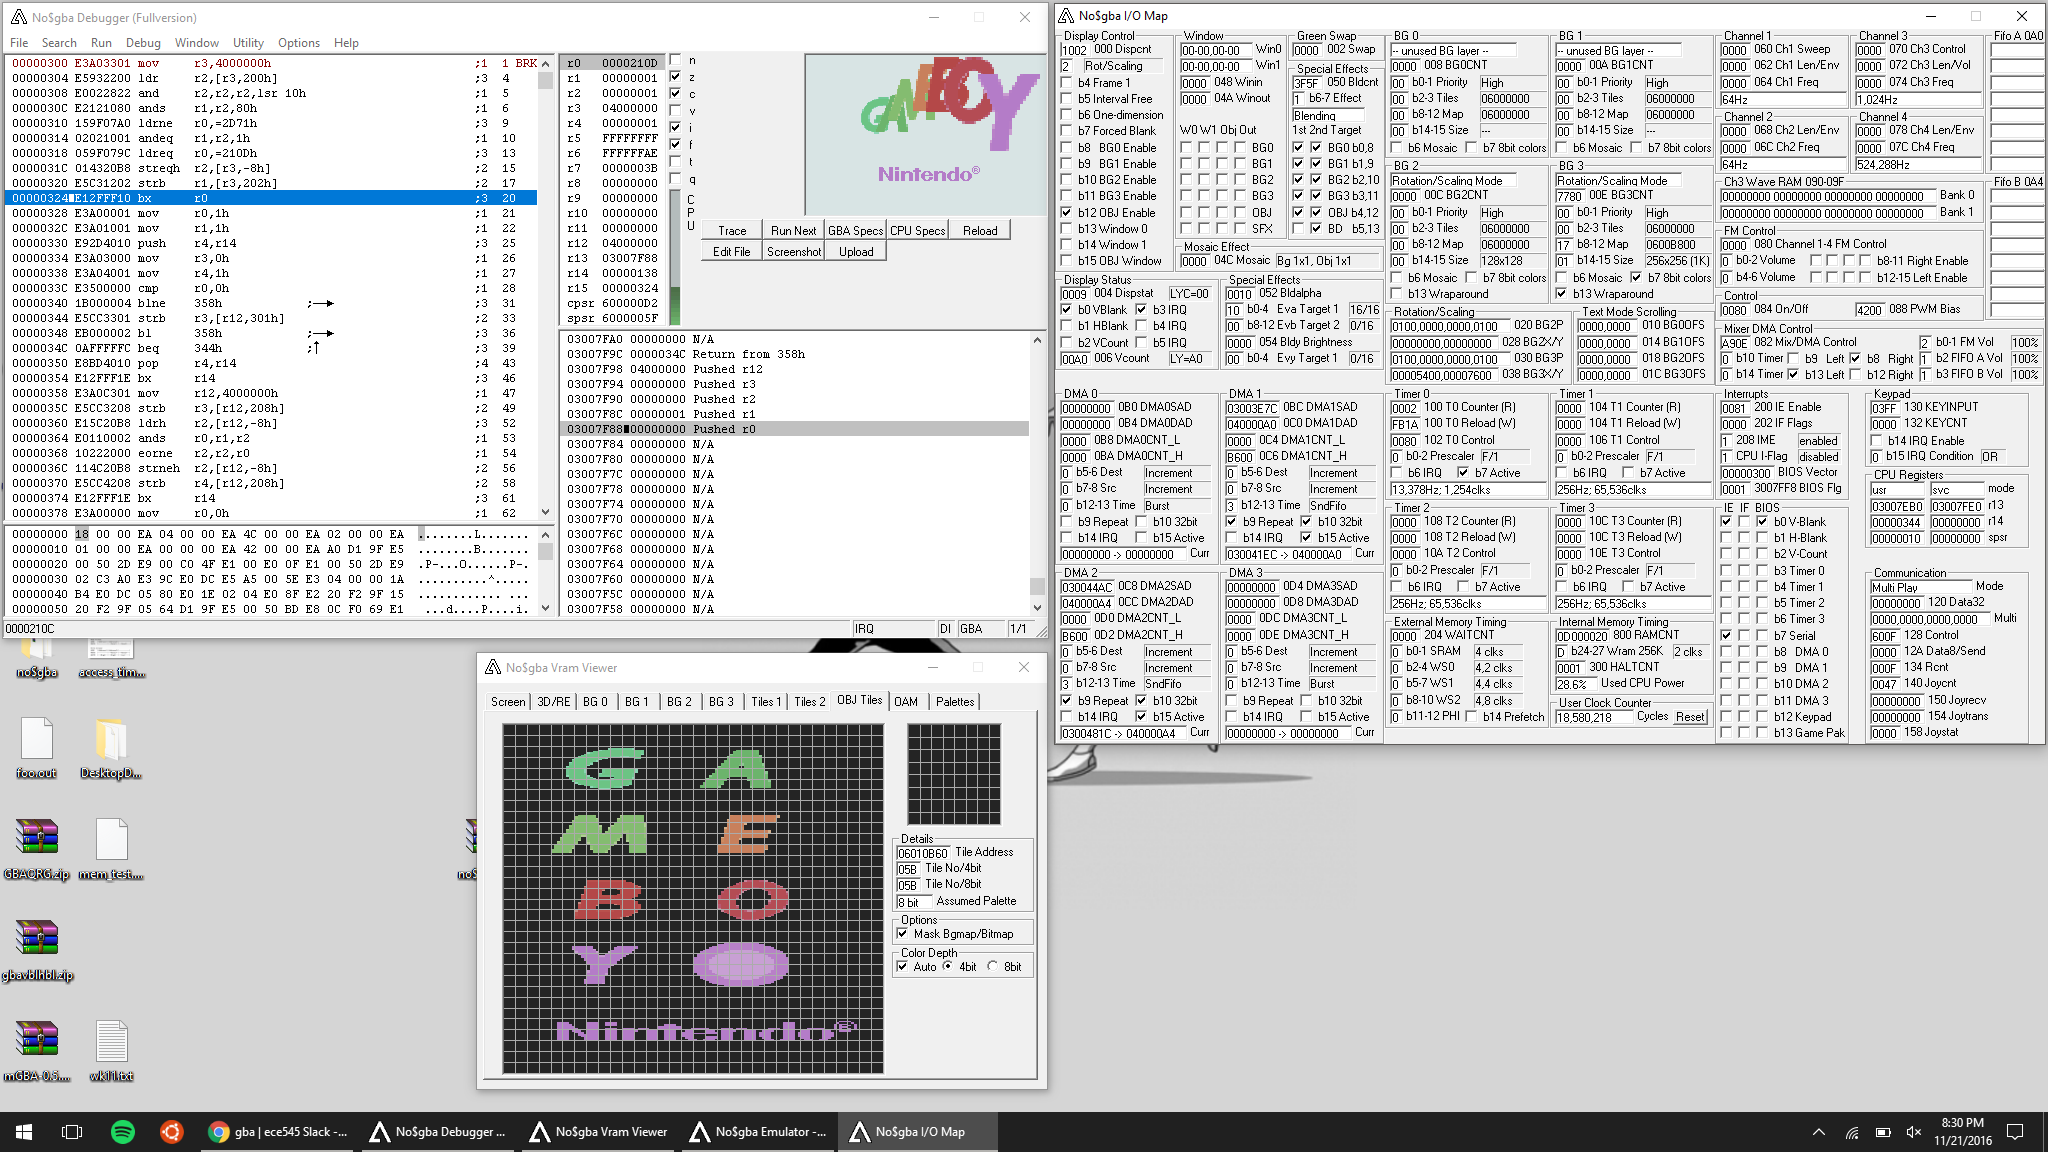
\includegraphics[width=12cm, height=10cm, keepaspectratio=true]{nogba}
	
	\section{Memory}
	A word on the GBA is defined as 32-bits, a half-word is 16bits. The Game Boy Advance memory is divided into 11 regions:\\
	\textbf{System ROM}: Mapped from \texttt{0x00000000} to \texttt{0x00003FFF}. Holds the GBA BIOS.\\
	\textbf{CPU External RAM}: Mapped from \texttt{0x02000000} to \texttt{0x0203FFFF}.\\
	\textbf{CPU Internal RAM}: Mapped from \texttt{0x03000000} to \texttt{0x03007FFF}.\\
	\textbf{I/O Registers}: Mapped from \texttt{0x04000000} to \texttt{0x04000807}. MMIO register mappings.\\
	\textbf{Palette RAM}: Mapped from \texttt{0x05000000} to \texttt{0x050003FF}. Stores the color palette.\\
	\textbf{VRAM}: Mapped from \texttt{0x06000000} to \texttt{0x06017FFF}. Video RAM.\\
	\textbf{OAM}: Mapped from \texttt{0x07000000} to \texttt{0x070003FF}. Object (sprite) attribute memory.\\
	\textbf{Game Pak ROM, WS0}: Mapped from \texttt{0x08000000} to \texttt{0x09FFFFFFF}. Cartridge ROM.\\
	\textbf{Game Pak ROM, WS1}: Mapped from \texttt{0x0A000000} to \texttt{0x0BFFFFFFF}. Cartridge ROM.\\
	\textbf{Game Pak ROM, WS2}: Mapped from \texttt{0x0C000000} to \texttt{0x0DFFFFFFF}. Cartridge ROM.\\
	\textbf{Game Pak RAM}: Mapped from \texttt{0x0E000000} to \texttt{0x0E00FFFF}. Cartridge RAM.\cite{GBAManual}\\
	Additionally, the upper 1M-bit of each ROM region is used as flash memory (presumably for game saves).\\\\
	Memory from \texttt{0x04000000} to about \texttt{0x04000807} is mapped to I/O registers (the programmers manual only lists register mappings up to \texttt{0x04000208}, but hobbyist reverse engineering shows some internal registers up to location \texttt{0x04000800}).\\\\
	VRAM is split into three regions: VRAM\_A\{\texttt{0x06000000 - 0x0600FFFF}\}, VRAM\_B\{\texttt{0x06010000 - 0x06013FFF}\}, and VRAM\_C\{\texttt{0x06014000 - 0x06017FFF}\}. Palette RAM is split into two regions bg\_palette\_ram\{\texttt{0x050000000 - 0x050001FF}\} and obj\_palette\_ram\{\texttt{0x050000000 - 0x050001FF}\}. In graphics, the system expects to be able to read from all 5 of these regions in each cycle - the memory controller needs to allow for this. Additionally, our graphics system required that we be able to read two values from VRAM\_A at once, though this is not strictly required by the architecture. \\\\
	In the process of booting the system, the BIOS checks that a valid ROM is inserted by checking that the byte \texttt{0x96} is stored in memory at location \texttt{0x080000B2} and that memory locations \texttt{0x0BFFFFE0 - 0x0BFFFFFF} are defined as halfwords \texttt{0xFFF0, 0xFFF1, 0xFFF2, ..., 0xFFFF}. Memory controller implementations that do not have a valid ROM mapped in memory need to emulate this behavior.\\\\
	Memory regions are also mirrored across 24-bit boundaries, along their size. For example
	The three regions for Game Pak ROM are identical mappings, the difference is the number of wait states used in the access (see Memory Interface). We used the Zedboard's BRAM for every memory region except CPU External RAM and GamePak ROM. Originally it would've been possible to fit External RAM into BRAM, but the double buffer for graphics took up the BRAMs that we would have used. We planned to use the Zedboard's DDR3 RAM for the Game Pak ROM, the Game Pak RAM, and the CPU External Working RAM, but we didn't have time to implement it. MMIO registers will be implemented with the Zedboard fabric SRAM.
	
	\subsection{DRAM}
	Since the Zedboard only has so much BRAM, and asking for the requisite 32MB of BRAM to fit a cartridge is a tall order for any board, we had planned to stored the GamePak ROM and CPU External RAM (also referred to as "On-board RAM") in the Zedboard's DRAM. Since there isn't a way to initialize DRAM upon board reset, our plan was to store the GamePak on an SD card, then, at system reset, have the SD card controller write the contents of the SD card to DRAM. Given that the CPU's clock is only at 16.78Mhz, we would be able drive our DRAM controller with a sufficiently fast clock to make DRAM accesses appear single cycle from the CPU's perspective. This, as it turns out, is surprisingly difficult to implement. The SD card on the Zedboard is only connected to the ARM core, meaning that the programmable logic can not actually interface with the SD card.  We were able to set up a Vivado SDK project that would read from the SD card on reset and write to BRAM using an AXI bus.  Unfortunately we were never able to properly set up a DRAM controller for the SD card to write to.  We planned to create an AXI master using HLS, that would write to DRAM, however we were unsuccessful.  We ran out of time, and had other more pressing priorities, to fully learn how to debug the AXI bus.
	 
	\subsection{Memory Regions Bus Widths}
\begin{center}
	\begin{figure}[ht!]
	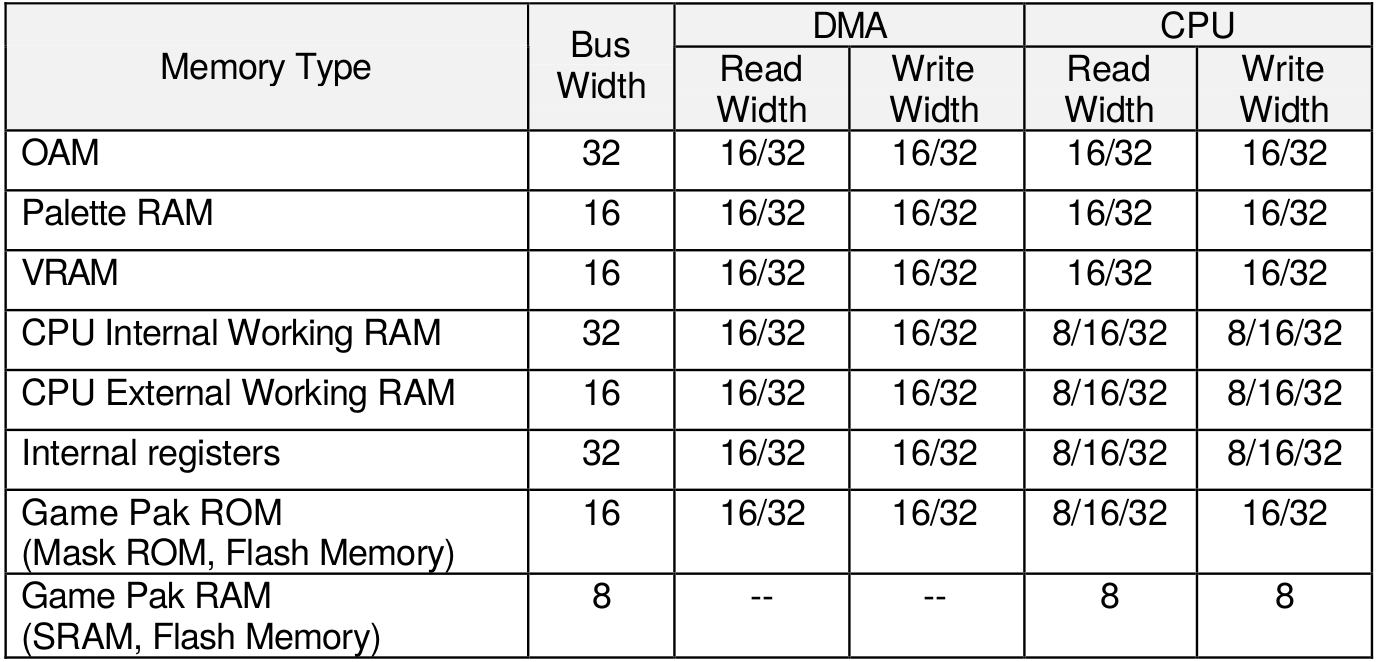
\includegraphics[height=6cm, keepaspectratio=true]{accesstimes}
	\end{figure}\cite{GBAManual}
\end{center}


	\subsection{Memory Interface}
	The memory interface is a bus, shared by the DMA controller and the CPU. Bus contention is avoided by priority - if a DMA is ready, the CPU is paused until the DMA completes. Neither the CPU nor the DMA can write to VRAM, OAM, or Palette RAM until either \texttt{VBLANK} or \texttt{HBLANK} regions of the VGA cycle. Outside of \texttt{VBLANK} or \texttt{HBLANK}, the graphics pipeline assumes exclusive ownership of VRAM, OAM, and Palette RAM, and the CPU/DMA bus is electrically disconnected (High-Impedence) from the graphics memory. During \texttt{VBLANK} and \texttt{HBLANK}, the CPU/DMA bus drives the bus for graphics memory as well.\\\\
	Bus accesses are sent to the memory controller, where they are forwarded to the memory region in which the address lies. If a system attempts to make an access to an undefined region, either the system will enter an error state, or the bus \texttt{ABORT} signal will be set high, depending on whether our target games make accesses to undefined regions during standard operation. If the latter is the case, we also have the option of mirroring undefined addresses onto defined regions (a step that the GBA does internally, but that isn't documented in the programmer's guide). The system is little endian.\\\\
	In our architecture, since BRAMs are dual ported, the CPU/DMA bus is allowed to write to graphics memory outside of \texttt{VBLANK} or \texttt{HBLANK}. In an ideal system, our memory controller would trigger an \texttt{ABORT} or some other error signal if graphics memory was written to outside of \texttt{VBLANK} or \texttt{HBLANK}, but we didn't have time to add this functionality. \\\\
	The various memories have different bus widths - to accommodate, the bus includes a \texttt{SIZE[1:0]} - where 3 corresponds to a word (32 bits), 2 to a half word (16 bits), and 1 to a byte (4 is reserved). When reading, the lowest two bits of the address will be used to determine the specific memory location, when writing, the combination of the lowest two address bits and \texttt{SIZE[1:0]} will be used to address specific locations.\\\\
	Our architecture gives the graphics pipeline direct access to address and read data ports of the BRAM. The CPU/DMA bus has the following signals:
		\begin{itemize}
			\item ADDR[31:0]  - address of the memory access (bottom 2 bits ignored for reads)
			\item RDATA[31:0] - Data read from memory location
			\item WDATA[31:0] - Data to write to memory location
			\item WRITE       - Write enable; Memory controller determines byte write enable by ADDR[1:0] and SIZE
			\item SIZE[1:0]   - Size of memory write {0 => byte, 1 => halfword, 2 => word, 3 => illegal}
			\item PAUSE       - Output. Pause the unit generating the memory access.
		\end{itemize} 

	
	\subsection{Memory Timings}
	Each region of the memory also has a specific access time. Specifically, this is where the three Game Pak ROM regions differ, in the case of the first region, WS0 denotes that zero wait states should be used in the access, for the second, WS1 denotes that one wait state should be used in the access, and so on. The length of a wait state depends on the state of the \texttt{WAITCNT} MMIO register. In the GBA system, accesses also recieve a speedup when they are sequential. We never planned to implement this, since DRAM and BRAM both give single cycle access. If it turned out that the timing differences are necessary for standard operation, we could have implemented delays for random accesses by asserting the \texttt{WAIT} bus signal as necessary. Different regions of GBA memory also have different access times associated with them - our plan of action was the same for this. Read and Write timings for our system are detailed below.\\\\
	Read Access:\\
		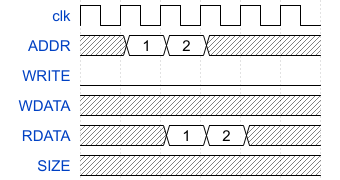
\includegraphics[height=4cm, keepaspectratio=true]{readaccess}
		\\
	Write Access:\\
	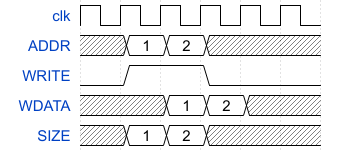
\includegraphics[height=4cm, keepaspectratio=true]{writeaccess}
	\\\\
	The difference between access timings for writes in our memory system (where write data is presented the cycle after write is asserted) and access timings for BRAMs (where write data is presented on the cycle that write is asserted) was fixed in our system adding several registers to delay address, write, and size by a cycle. This creates a bit of a problem - if a write is immediately followed by a read, both will try to present an address to the BRAM on the same cycle. See the diagram below - W corresponds to the memory write, R corresponds to the memory read. We solved this with a slight hack - \texttt{PAUSE} is asserted on every write. It would behoove future groups to redesign the controller to avoid this - it would make it easier to adhere to GBA memory region access timings.
	

		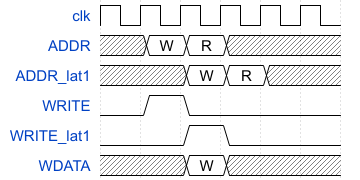
\includegraphics[height=5cm, keepaspectratio=true]{badaccess}


	Additionally, with system as described as above, each write will occur twice with the same address and data. Normally, this is fine, but each write will count as two words written to the Direct Sound FIFO. This is only a problem in our system during the \texttt{STM} instruction where \texttt{WRITE} is asserted for multiple consecutive clock cycles. Our fix was specific to this case, the write enable for the BRAM is only asserted if \texttt{PAUSE} wasn't asserted in the previous cycle. Again, this is a bit of a hack - it would be prudent to implement a fix into the actual design for the memory controller.\\\\

	\subsection{Memory Region Access Timings}
	\begin{verbatim}
	    Region        Bus   Read      Write     Cycles
	    BIOS ROM      32    8/16/32   -         1/1/1
	    Work RAM 32K  32    8/16/32   8/16/32   1/1/1
	    I/O           32    8/16/32   8/16/32   1/1/1
	    OAM           32    8/16/32   16/32     1/1/1 *
	    Work RAM 256K 16    8/16/32   8/16/32   3/3/6 **
	    Palette RAM   16    8/16/32   16/32     1/1/2 *
	    VRAM          16    8/16/32   16/32     1/1/2 *
	    GamePak ROM   16    8/16/32   -         5/5/8 **/***
	    GamePak Flash 16    8/16/32   16/32     5/5/8 **/***
	    GamePak SRAM  8     8         8         5     **
	    Timing Notes:
	    *   Plus 1 cycle if GBA accesses video memory at the same time.
	    **  Default waitstate settings, see System Control chapter.
	    *** Separate timings for sequential, and non-sequential accesses.
	    One cycle equals approx. 59.59ns (ie. 16.78MHz clock).
	    Sequential vs Random access timings on p.23 of Nintendo GBA doc
	    All memory (except GamePak SRAM) can be accessed by 16bit and 32bit DMA.
	    \end{verbatim} \cite{GBATek}
	

	\section{CPU}
	\subsection{Overview}
	The GBA uses an ARM7TDMI processor, implementing the ARMv4t ISA, which operates on a three-stage pipeline (fetch, decode, execute). When an instruction in the execute stage will take more than one cycle to complete, the CPU stalls the pipeline until the instruction completes. For branches, the CPU flushes the fetch and decode stages, reloading from the address that was branched to. The CPU also (per ARM specification) can switch between 32-bit ARM instruction mode and 16-bit THUMB instruction mode via the \texttt{BX} instruction. During execution, the program has accesses to 17 registers, with R13, R14, and SPSR swtiched between several banks depending on execution mode.\\\\
	We had planned to get most of the CPU from an outside source, then implement the necessary features. Our options were either the Storm Core from OpenCores, the ARM9 chip embedded on the Zedboard, or a version of the ARM7TDMI that some engineer wrote between jobs. Interestingly, the core from some random engineer seemed the most promising since THUMB mode was partially implemented already. The Storm Core had no infrastructure for THUMB mode in place, as well as some other issues, and the ARM9 core had some backwards compatibility issues between ISA versions that we wouldn't be able to implement hardware fixes for.\\\\
	As we learned, getting the interactions between THUMB mode and ARM mode, especially at the points where the CPU switches between them is extremely tricky, especially when working in the context of a core that someone else wrote. All in all, getting the CPU to a working state took about 12 weeks of debugging 40+ hours a week. Currently, the CPU runs an unmodified BIOS perfectly, as well as several games that we tested, mostly written by outside sources. A warning to future groups - there may still be bugs in the CPU that need to be fixed to run commercial games, but they should mostly be fleshed out.\\\\
	As a guide, since a decent portion of the core remains unmodified from original version, a short list of helpful information and documentation is below. It likely won't be enough to completely understand the system, but it should be enough to get started.\\\\
	The CPU has 6 execution modes: Fast Interrupt (FIQ), Interrupt (IRQ), Undefined Instruction (UNDEF), Supervisor (SVC), Memory Abort (ABORT), and User (USER). Per the ARM specification, there should also be System Mode (think kernel mode in x86) where memory accesses to certain regions and writes to certain registers are unrestricted, but this and User mode are treated the same in this implementation.\\\\
	In our implementation of the GBA, DMA can pause the CPU to preempt it so that DMA can take control of the memory bus. To avoid this preemption interrupting multi-cycle execute instruction or branches, we added a \texttt{preemptable} output that signals to DMA when the CPU can be preempted. Since multi-cycle instructions stagnate the pipeline (signal \texttt{StagnatePipeline} and \texttt{StagnatePipelineDel\_Int} in \texttt{ControlLogic.vhd}) and branches refill the pipeline (with signal \texttt{PipelineRefilling} in Instruction Pipeline/Data In register (\texttt{IPDR.vhd})), the CPU is preemptable when none of the signals listed above are asserted.\\\\
	During normal program execution, PC (\texttt{REGFILE\_INST.UM\_REGISTER\_FILE(15)}) points to the address of the instruction that is currently in the Fetch stage of the pipeline, which is either 8 or 4 greater than the address of the instruction that is currently in the execute stage of the pipeline, depending on whether the CPU is in ARM or THUMB mode. \texttt{ADDR} points to the next instruction to be fetched, either PC+4/PC+2, or the target of a taken branch or a jump.\\
	
	\subsection{Pipeline Overview}
	The core has three pipeline stages - Fetch, Decode, and Execute. Since accesses to memory have a 1 cycle latency, RDATA acts as the register for the instruction in the Fetch stage. In the case of instructions that are multi-cycle in the Execute stage and present addresses to memory, the Fetch stage instruction (and relevant signals) will be stored in the \texttt{PrefetchedInstruction} register in Instruction Pipeline/Data In register (\texttt{IPDR.vhd}) until the end of the multi-cycle instruction, then muxed into Decode stage registers.\\\\
	The Decode stage instruction is output from the Instruction Pipeline/Data In register (IPDR, \texttt{IPDR.vhd}), through the THUMB Decoder (\texttt{ThumbDecoder.vhd}). The THUMB Decoder, if the CPU is in THUMB mode, determines which half of the 32-bit word is the instruction for the current cycle from \texttt{HalfWordAddress}, then translates the THUMB instruction into a 32-bit ARM instruction. If the CPU is in ARM mode, the instruction is passed through unchanged. From the THUMB Decoder, the instruction is sent back to the IPDR then to \texttt{ControlLogic.vhd}, where the \texttt{IDC\_*} signals are set based on what type of instruction it is.\\\\
	For the Execute Stage, all \texttt{IDC\_*} signals are passed to the same \texttt{IDR\_*} signal. The ALU computes on the values on the ABus and the BBus, which are set by the ABusMultiplexer (\texttt{ABusMultiplexer.vhd}) and BBusMultiplexer (\texttt{BBusMultiplexer.vhd}), respectively. The output of the ALU is wired to the input of the Program Status Registers (CPSR, SPSR in \texttt{PSR.vhd}) and the input of the Result Bit Mask (\texttt{ResItBitMask.vhd}) where, selectively, bit 0 is cleared/set and bit 1 is cleared, based on signals from \texttt{ControlLogic.vhd}. The output of the Result Bit Mask is an input to the Address Mux (\texttt{AddressMux\_Incrementer.vhd})and the Register File (\texttt{Regfile.vhd})
	
	\subsection{THUMB Mode}
	In THUMB mode, instructions are 16-bits instead of 32-bits long. THUMB instructions, however, are a subset of ARM instructions. Since CPU size wasn't a design concern, and THUMB mode was unimplemented in the core we started with, instructions go through a Decoder that translates the THUMB instructions into equivalent ARM instructions, so they can be passed to the Decode stage of the processor as ARM instructions. In reality, the ARM7TDMI likely uses muxes on each signal in the decode stage, either using the signal from the ARM decoder or the THUMB decoder based on the CPU mode, but implementing the Thumb Decoder this way allowed for minimal modifications (and didn't require a complete understanding of the processor).
	
	\subsection{Branches}
	On a high level, there are three types of branches: Normal branches, Branch and Link (BL), and Branch and Exchange (BX). In ARM mode, branches specify a 24-bit offset relative to the value that PC will have when the branch is in the execute stage of the pipeline. The offset is shifted left by two bits, then added to PC (which is the address of the branch plus 8) to get the target. In THUMB mode, the offset is shifted left 1 bit and added to the PC (which is the address of the branch plus 4).
	
	\subsubsection{Branch and Link}
	In ARM mode, Branch and Link instructions in ARM operate the same as normal branches, but store the return address (current PC plus 4) in R14. In THUMB mode, branch and link instructions occur over two instructions. The first instruction in the BL 
	causes the bottom 11 bits of the instruction to be stored in the \texttt{ThBL\_Reg} register in \texttt{ThumbDecoder.vhd}. The second instruction's offset minus 1, shifted left 1 bit is added to the value in \texttt{ThBL\_Reg} shifted left by 12 bits to get the BL offset, which is passed to the ARM decoder as a BL instruction. The first instruction in a THUMB BL is passed as a NOP to the ARM decoder. The ARM decoder doesn't shift Branch instructions in THUMB mode - the shifter control treats it as a default case. When we started work on the processor, two signals \texttt{ThBLFP} (THUMB BL First Part) and \texttt{ThBLSP} (THUMB BL Second Part) were outputs of the THUMB Decoder to account for BL in THUMB mode, but it was easier (and required fewer deep dives into the details of the processor) to write custom logic to handle this case. Timing diagrams are below: \textbf{B} denotes the branch instruction (or address) and \textbf{T} denotes the branch target instruction (or address). \texttt{IDR\_BL}, \texttt{BRANCH\_St1}, and \texttt{BRANCH\_St2} are signals in \texttt{ControlLogic.vhd}. \texttt{PipelineRefilling}, another signal in \texttt{ControlLogic.vhd}, is asserted when either \texttt{BRANCH\_St1} or \texttt{BRANCH\_St2} are asserted. In THUMB mode, the lowest bit of the return address is set - see Branch and Exchange.\\\\
	\newpage
	ARM Mode Branch and Link:\\
	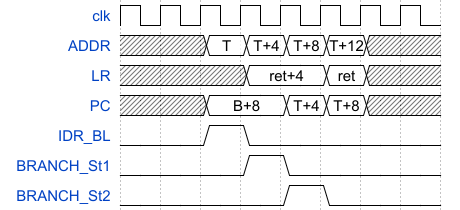
\includegraphics[height=4cm, keepaspectratio=true]{armbl}\\
	
	THUMB Mode Branch and Link:\\
	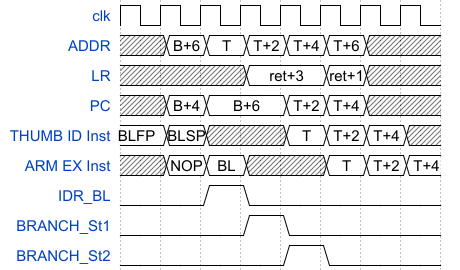
\includegraphics[height=6cm, width=8cm, keepaspectratio=true]{thumbbl}
	
	\subsubsection{Branch and Exchange}
	Branch and Exchange is the same between ARM and THUMB mode, except when the register being branched to is R15. ARM discourages this use, so, assume that BX is the same between modes. Branch and Exchange acts the same as a normal branch, with the same timings as detailed above (with \texttt{IDR\_BX} instead of \texttt{IDR\_BL}), except that the CPU mode is set based on the lowest bit of the register being branched to - THUMB mode if the lowest bit is 1, ARM mode otherwise.
	
	\subsection{Load/Store Timings}
	For the sake of clarity, below are access timings for a LDR (load register) and STR (store register) instruction. Both are good example of multi-cycle execute instructions. \textbf{M} refers to the load/store access, \textbf{Next} refers to the next instruction.\\
	LDR Timing:\\
	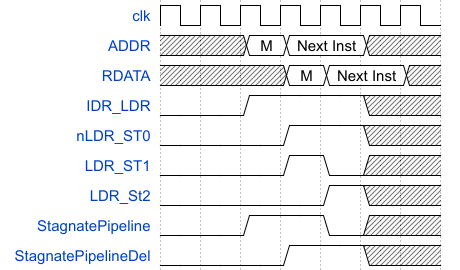
\includegraphics[height=6cm, width=8cm, keepaspectratio=true]{ldr}\\\\
	STR Timing:\\
	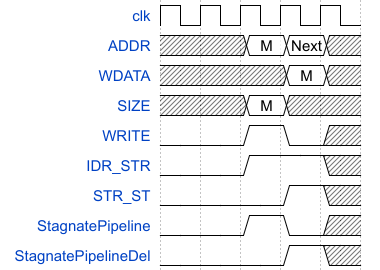
\includegraphics[height=6cm, width=8cm, keepaspectratio=true]{str}
	
	
	\subsection{Errata}
	Most fixes to the CPU that made it into the final implementation were done as cleanly as possible and should not be cause for future bugs. One fix, however, needed to be done less cleanly since time was running out in the semester. So, as a warning, the logic for \texttt{SngMltSel} - the select line on the output multiplexer in the Load Store Address Generator (\texttt{LSAdrGen.vhd}) - may be incorrect. The problem was that an STM after an LDR would have the wrong address, the fix was to add "and (not IDC\_STM)" to the end of the condition for \texttt{SngMltSel}. This fix felt like it might cause the instruction sequence STM, LDR to break the system, but that might just be paranoia. Either way, be careful. Additionally, the logic for \texttt{AdrIncStep} in \texttt{ControlLogic.vhd} caused 7 bugs. It seems to be working, but if it needs to be fixed in the future, be extremely careful - make sure that all the cases (LDM, STM, BX, etc.) are accounted for.
	
	\subsection{CPU Interface}
	The ARM7TDMI core that we got didn't have all the signals that are described in the ARM7TDMI specification. In fact, most of the signals were missing. The ARM7TDMI was a fairly popular processor, designed for a much more general purpose than the GBA, so many of the signals were unnecessary for our context. Namely, the JTAG debug interface (the D in TDMI), and the EmbeddedICE macrocell (the I in TDMI) were intended for post-silicon verification - a process that is wholly unnecessary for our project. The processor also allows for a choice between unidirectional and bidirectional data buses, which we also don't need - we picked unidirectional and stuck with it. We also don't use the coprocessor interface - it was used in the GBA to provide backwards compatibility with Game Boy Color games (interfacing with a Z80 processor). All in all, the signals that we actually need for our interface is an aggressive subset of the signals specified in the ARM7TDMI documentation - if the core we got online didn't have it and we could justify not including it, we didn't. We lose cycle accuracy, but that was never a primary goal of the project and it seems easier to adhere to approximate cycle timings in the context of our system than try to replicate cycle timings that we don't have access to. Again, the primary issue due to our lack of cycle accuracy is memory accesses occurring faster than they should, but we can add wait timings to try to replicate the original timings (or to get closer to them).\\\\\\
	The interface from the CPU to the rest of the system is as follows:
	\begin{verbatim}
	input  logic CLK,          		// The system clock
	input  logic PAUSE,        		// Pause the CPU when high (for wait states)
	input  logic DMAActive     		// Pauses CPU and sets memory output bus signals to 'Z
	input  logic nRESET,     		// System reset
	
	-- Interrupts
	input  logic nIRQ          		// Interrupt Request
	
	-- Memory interface
	output logic [31:0] ADDR, 		// Memory Address
	output logic [31:0] WDATA,		// Write Data
	input  logic [31:0] RDATA, 		// Read Data
	input  logic ABORT,       		// ABORT memory access
	output logic WRITE,        		// Write enable
	output logic [1:0] SIZE,   		// Memory write size
	
	-- Status Signals
	output logic [4:0] mode         // Current execution mode of the CPU
	output logic       preemptable  // If the CPU can be paused (so pauses are synchronous to the instruction stream)
	\end{verbatim}
	The module header for the core also includes a \texttt{FIQ} signal for fast interrupts, but the GBA doesn't use these. The signal's integrated in the logic for the core - it seemed like an unnecessary amount of work to remove it.
	
	\subsection{Testing}
	We put a fair amount of work into getting some sort of automated testing infrastructure for the CPU in simulation. This involved running a similar core to the ARM7TDMI in QEMU, attaching GDB to the QEMU process, printing out registers every cycle, and writing the output to a text file. The testbench for the CPU would also write register states to a text file every cycle. Both these files would be processed to give a list of register value changes, then the two resulting files would be diffed. \\\\
	This was helpful - it gave a decent level overview of where output differed, but took several days to setup and didn't end up being all that useful. For the most part, a bug in the CPU would either cause an infinite loop or the CPU to enter an undefined state, so looking for the first register value that differed wasn't needed to track down cause. Additionally, PC in the CPU always differs from PC in the emulation (since PC in the CPU actually points to two instructions ahead of the current instruction).\\\\
	In the end, we exclusively used NO\$GBA. There weren't any bugs where the CPU followed the same control flow and gave the wrong answer for some calculation, so doing a diff of register states by hand was enough. This was also after we moved the CPU onto the board - it took about 5 minutes to run a simulation of 135000 instructions of the CPU - there weren't a lot of other options.
	
	\subsection{Interrupts}
	The CPU has a single interrupt request line, but can receive interrupts from 14 different sources. This is managed via the Interrupt Controller, along with a couple MMIO registers. The CPU's nIRQ line is set to the OR of all incoming interrupts that have not been masked (masking in Interrupt Master Enable and Interrupt enable registers). When an interrupt is received, the CPU enters nIRQ mode, then examines the Interrupt Request (IF) MMIO register to determine the source of the interrupt. Interrupt priority is handled by software \cite{GBAManual}.\\\\
	An interrupt can be generated by the following sources:
	\begin{multicols}{3}
	\begin{itemize}
		\item GamePak (IF[13])
		\item Key Press (IF[12])
		\item DMA{0-3} Transfer (IF[11-8])
		\item Link Cable Communication (IF[7])
		\item Timer Overflow (IF[6-3])
		\item V Count match (IF[2])
		\item HBLANK (IF[1])
		\item VBLANK (IF[0])
	\end{itemize} 
	\end{multicols}
	
	Since our final design did not include a GamePak, we never looked into details of how GamePak interrupts are implemented, where interrupts are routing from, etc. Presumably, game specific hardware in the cartridge (like the real-time game clock in Pokemon Games) could interrupt the CPU, but we don't have a basis for this. Future groups should definitely look into this if they plan to implement game cartridges.\\\\
	As a note, if the \texttt{nIRQ} line is held low for too long, the CPU will enter into an undefined state. Our solution was to hold the line low until the CPU entered IRQ mode (shown by a change on the \texttt{Mode} output of the CPU), more elegant solutions likely exist. In any case, our interrupt controller likely has bugs - the BIOS only needs to generate interrupts on VBLANK to run; many interactions were untested.
	
	\section{DMA}
	The GBA has 4 DMA channels numbered 0 to 3. Only one DMA channel can be operating at once, so DMA channel 0 has the highest priority, 1 has the second, and so on. When a higher priority channel preempts a lower priority channel, the lower priority channel is paused until the higher priority channel completes. Preemption of a lower priority channel can not actually happen until it has finished its current read write sequence.  As mentioned before the DMA has priority of the memory bus and can pause the CPU, however preemption of the CPU can only happen synchronous to the instruction stream.\\\\
	Individual DMA channels differ slightly in expected use. DMA0, naturally, is used for high priority transfers (feeding graphics during HBLANK) and cannot be used to transfer from GamePak ROM, DMA1 and DMA2 can be used to feed DMA sound channels, and DMA3 can be used to transfer data from GamePak ROM.\\\\
	For each DMA, the source address is specified in MMIO \texttt{REG\_DMA*SAD}, the destination address in \texttt{REG\_DMA*DAD}, the number of words or half-words to transfer in \texttt{REG\_DMA*CNT\_L[13:0]}.
	General controls are set in \texttt{REG\_DMA*CNT\_H[15:0]}, including whether the count is the number of words or half-words, whether the transfer will repeat, when the DMA will start, enables, and whether the DMA will generate a CPU interrupt upon transfer completion ~\cite{GBAManual}.
	
	\section{Graphics}
	The Game Boy Advance graphics pipeline uses a combination of backgrounds and sprites, which the GBA refers to as objects. There are three types of backgrounds - Character backgrounds, where the screen is composed of tiles that specify colors in a palette, Rotation/Scaling backgrounds, where the screen is tiled, but the tiles can be scaled or rotated (but fewer can be used), and Bitmap backgrounds, where the entire screen is specified pixel-by-pixel with colors specified in a palette. All backgrounds can be flipped vertically or horizontally. The background mode (specified in DISPCNT) controls how many backgrounds, and which types of backgrounds, can be used. \cite{GBAManual}
	
	\subsection{Objects}
	Objects are stored in character mode, where pixels index into a palette for color values. Limits on objects, like the number of objects that can display and which palettes are used, are determined by the background mode. Parameters for objects are specified in OAM in sets of 4 bytes, or 2 bytes when using bitmapped backkgrounds (Background mode 3-5). Objects are given a priority (from 0-3) as part of the parameters, with 0 taking the highest priority. \cite{GBAManual}
	
	\subsection{Priority}
	Objects with priority 0 have the highest priority. Backgrounds with priority zero are next, then objects with priority 1, then backgrounds with priority 1, and so on. The backdrop has the lowest priority, which is just a default color if the color for a given pixel are unspecified. If objects or backgrounds are transparent, the transparent color (color 0) is used (specified in the palette). \cite{GBAManual}. 
	
	\subsection{Windowing}
	The Game Boy Advance has a notion of windows, where objects and backgrounds inside the windows can be collectively turned on or off. The size and location of the windows are set in MMIO registers. Window 0 has a higher display priority than window 1. \texttt{REG\_WININ} is used to control whether BG3, BG2, BG1, BG0, or objects are turned on or off. \cite{GBAManual}
	
	\subsection{Mosaics}
	Backgrounds and sprites can be drawn with a mosaic, where some number of dots of a normal display should comprise a large dot. Specifically, starting from the top-left corner, a block of size \{H size * V Size\} will be the same color as the top-left corner. This has the effect of dividing the screen into \{H size * V Size\} chunks, where blocks on the edges will be smaller if the background/object can't be evenly divided into chunks. All background are set to the same mosaic size (if one is specified), the same holds for all sprites. Mosaic information is specified in \texttt{REG\_MOSAIC}.\cite{GBAManual}
	
	\subsection{VGA Display}
	Natively, the GBA expects a 240x160 resolution - a 3:2 aspect ratio. This doesn't exist in modern monitors. Originally, we had planned to output 480x640 VGA, but the GBA documentation didn't give us pulse width timings. In the end, we decided to double buffer the display, storing the double buffer in the Zedboard's BRAM. The graphics pipeline writes the color data that will be output to the double buffer controller and asserts that the buffers should switch at the end of a display cycle (\texttt{toggle}). The VGA controller presents the buffer address for the next pixel (since reads are sequential from BRAM) and writes the data read from the buffer to \texttt{VGA\_R[3:0], VGA\_B[3:0], VGA\_G[3:0]}. The VGA is clocked at three times the system clock (16.78Mhz), so that both the VGA controller and the graphics pipeline stay coordinated on a per-frame basis. 
	
	\section{Audio}
	The GBA has four wave sound channels and two DMA sound channels. The wave channels are identical to the Game Boy Color, with each channel having slightly capabilities. Channel 1 generates a square wave tone with optional frequency sweep, channel 2 generates a rectangular tone, channel 3 generates a sawtooth wave, and channel 4 generates white noise. The frequency sweep in channel 1 is not implemented in our design, because it requires updating the SOUND1CNT\_X with new updated frequency values.  None of the games in our demo used a frequency sweep, so this piece of integration was not something that took priority.  Channel 1 and 2 are implemented with a square wave module that generates the square wave, the square wave then gets passed through a length counter that cuts stops the square wave at the given length.  Lastly the square wave gets passed through a volume envelope, that changes the volume at a specific rate.  Channel 3 is implemented with a wave channel, that reads the sound data from WAVE\_RAM0-3 and then sends it through a length counter before sending it to the sound circuit.  Lastly, channel 4 creates a noise wave using a linear feedback shift register (LFSR) to generate a pseudo-random bit sequence.  The noise channel then passes through a volume envelope and length counter.  Each of the 4 channels above also has a clock divider, because the volume envelope is clocked at 64 MHz and the length counter is clocked at 256 MHz.\\\\
	Direct sound was a new feature added to the GameBoy Advance to add more sound control, over simply mixing together 4 channels of sound. Games could now put streams of 8 bit sound data into memory, and schedule it to play without any more CPU interaction.
	The two direct sound channels can be configured to use any combination of the two timers, and two DMA channels. The given timer is set to choose the number of cycles between samples. On every timer overflow the audio data is passed from a FIFO to the mixer. When the FIFO has only 4 words left, a request will be made to the DMA channel to transfer four more words of data to the FIFO. The FIFO has a maximum depth of 8 32-bit data and is written to directly when the DMA channel writes to the Sound FIFO Input MMIO register. The mixer varies the volume, and ratio of direct sound to 4-channel sound, then outputs to the sound circuit. ~\cite{GBAManual}.
	
	\subsection{Zedboard Audio Codec}
	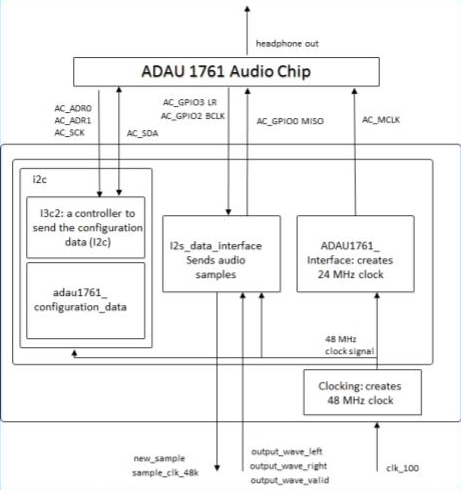
\includegraphics[width=14cm, height=15cm, keepaspectratio=true]{newcodec}
	The sound circuit[1] uses an I2C interface to configure the ADAU1761 Audio Chip on the Zedboard.  The audio is then transmitted to the chip using I2S.  The sampling rate at which data is passed to the audio chip is 48KHz.
	
	\section{Timers}
	The Game Boy Advance, per specification, has 4 16-bit timers that are programmed via registers TM{0-3}CNT\_{L,H}. These timers can be programmed to count at the system clock rate, or at 1/64th, 1/256th, or 1/1024th of the system clock rate. Each timer can also generate an interrupt when the timer count overflows the 16 bit TM{0-3}CNT\_L register. The counter just changes its current value in the given MMIO register at the specified rate.  If interrupts are not enabled, other modules have to poll the register to see when the timer has overflowed.  Multiple timer registers can be added together to allow for longer timing delays by setting count-up timing, which only allows timer X+1 to start counting after timer\_X completed.\\
	
	\section{Controller}
	We use an SNES controller connected to one of the Zedboard's PMOD ports. The controller is connected as follows:
	\begin{verbatim}
	       ----------------------------- ---------------------
	       |                             |                      \
	       | (1)     (2)     (3)     (4) |   (5)     (6)     (7) |
	       |                             |                      /
	       ----------------------------- ---------------------
	       
	       Pin     Description             Zedboard Connection
	       ===     ===========             ======================
	       1       +5v                     Zedboard +5V
	       2       Data clock              JA3
	       3       Data latch              JA2
	       4       Serial data             JA1
	       5       ? (+5v)                 no wire
	       6       ? (+5v)                 no wire
	       7       Ground                  JA GND
	\end{verbatim}
	As detailed above, the Zedboard expects a +5V VDD, whereas the PMOD connectors output at +3.3V. To avoid frying the Zedboard, we used a \textit{Sparkfun Level Converter}. As a note, to properly use the level converter, ground on either side should be connected to ground on the Zedboard (either one of the ground pins, or ground on one of the PMOD connectors), +:q3.3V should come from the PMOD connector, and +5V should come from the 5V pin on the Zedboard.\\\\
	The serial protocol between the controller module on the Zedboard and the SNES controller begins with the CPU sending a 12us wide positive pulse on the Data Latch pin. The CPU wait 6us, then sends 16 data clock pulses, beginning with the negative edge of the clock, that are 50\% duty cycle with a 12us period on Data Clock (Data Clock is high when idle). The Controller shifts latched button states on the positive edge of the Data Clock, and the CPU samples the Serial Data line for button state on the negative edge. Button state is reported active-low. In our implementation, button state is reported in the order below:\\
	\begin{verbatim}
    Clock Cycle     Button Reported
    ===========     ===============
    1               B
    2               Y
    3               Select
    4               Start
    5               Up on joypad
    6               Down on joypad
    7               Left on joypad
    8               Right on joypad
    9               A
    10              X
    11              L
    12              R
    13              none (always high)
    14              none (always high)
    15              none (always high)
    16              none (always high)
	\end{verbatim}
	The serial protocol repeats at 60Hz. The GBA buttons register expects (from low to high) \{A, B, Select, Start, Right, Left, Up, Down, R, L\}, so we reorder the outputs in our controller module.
	
	
	\subsection{Status \& Future Work}
	At demo day, our system ran the BIOS and booted one of two different ROMs: \textit{WolfARMStien} - a 3-D maze to explore in the style of Wolfenstien (written by an outside source), and \textit{Nintendo Pong} - a version of Pong with Mario and Luigi as paddles and a Pokeball as the ball. The system ran without any processing bugs, however the visuals were still a bit glitchy. Everything was, however, deterministically gitchy which means our system was stable, if nothing else. DMA sound played for the BIOS, but was a bit choppy. \textit{Nintendo Pong} used 4 channel sound, which was identical to an emulator.\\
	
	
	\section{Vivado Tips and Tricks}
	Unpopular opinion time: Vivado is a pretty good piece of software. Synthesis runs can be upwards of 20 minutes for full system implementation, but considering that an entire GBA is being synthesized, this is perfectly reasonable. However, it can be quirky in some cases. Like VCS, Vivado is the only program for compiling to the Zedboard, so many features aren't as polished as they could be. For instance, disconnecting the programming cable while an ILA is active will cause Vivado to segfault - fun for a security researcher, less fun for computer engineers. Like it or not, though, Vivado is what every 545 group will likely be using. With that in mind, a few tips:\\\\
	ILAs can either be created by selecting nets after synthesizing a design (in "Synthesized Design") or by using an ILA IP block. The latter will have faster compilation times for implementation, but will required re-generating the IP block if the number of signals or width of signals changes. It also needs to be wired up by hand, which can make debugging large numbers of signals tedious. Selecting nets in a synthesized design gives much more flexibility in choosing debug nets. As a note: nets in "Synthesized Design" will not always (and will often not be) named the same as in the source code. To guarantee consistent name resolution, prefix a signal declaration for a signal that will be debugged with "(* mark\_debug = "true")" in System Verilog, or add the line "attribute mark\_debug of <signal\_name> : signal is "true";" in VHDL (with "attribute mark\_debug : string;" at the top of the VHDL file). We recommend this method - signals will be auto-selected for debug cores and can be removed on a per-run basis. During integration, we regularly had 1500+ signals in an ILA so we could work on multiple bugs per synthesis run.\\\\
	We had issues using Block Memory Generators with 32-bit address interfaces - mappings to data weren't working as they should. It's easier to just have address lines only as wide as necessary for the memory and add some extra logic.\\\\
	Vivado is pretty bad with source control and transferring projects between systems, especially with IP cores. As a "nuclear option" an entire project can be exported as a ZIP archive and reopened on another machine. Adding all the files in a vivado project to Git is an option, but a bad one - commits will give thousands of lines over dozens of files. Vivado also dumps a bunch of files in the directory that it's run in (vivado\_*, webtalk\_*, etc.). These can be safely deleted, but they're a bit annoying.\\\\
	Vivado is also a bit weird with inferring clock domains, as well as inferring which signals are clocks. If possible, never implement clock dividers from scratch, just use the Clock Generator IP block. Also, if possible, only use one Clock Generator for all clocks - switching to this fixed a couple non-deterministic bugs in our system. Only clock registers off of signals coming from the clock generator module.\\\\
	Many Vivado warnings, like "always\_comb does not infer combinational logic" should probably be errors or, at least critical warnings. In fairness, Quartus labels similar things only as warnings. Our advice is this: if a system is buggy, the first step should be to look at Vivado warnings. Every warning from synthesizing a project should be looked into. If finding the source of the warning (or inferred latch) is difficult, VCS sometimes gives better descriptions of where the problem is. 
	
	\section{Lessons Learned}
	System integration without a CPU is not really possible, so it is extremely valuable to get a working CPU fast.  In order to leave enough time for system integration every part of the project should be completely done well before the deadline.  Future teams attempting the GBA project should use our ARM core. \\\\
	Fixing bugs in a system without understanding everything leads to more bugs, which then leads to fixing the same line of code over and over again.\\\\
	When starting the project if you are completely lost and everything seems magical, it's probably pretty simple all the way down.  Just start with one small piece at a time until the project starts building on itself.\\\\
	We ran into problems were the spec was ambiguous, so we just made assumptions on what should happen.  We would figure out if our assumption was wrong during integration.  However, because integration did not happen until a long time afterward, it took some time to remember what assumptions were made.\\\\ Testing understand of a spec after reading it with writing custom games is a good idea.\\\\
	Schedules and Gant Charts are nice for reassuring people that everything will be done on time. They aren't good for much more than - most assumptions about how long things will take will be wrong, especially with a project of this complexity. Having an idea about what will get done in the coming week is good - there isn't any need to plan farther than that in advance. \\\\
	
	\section{Personal Statements}
	\subsection{Rachel}
	
	\subsection{Steven}
	
	\subsection{Neil}
	
	
	\section{Future Groups}
	This is a very doable project for a determined group that wants to play Pokemon Ruby or any other fantastic game made for the GBA. Please, please, please, please use our CPU. Not being able to actually start system integration until the CPU was done (which was after Thanksgiving) puts a project on precarious grounds - no one has any idea if anything will actually work until the last week. Read this report several times, we worked hard to give as much useful information as possible. Then, read Nintendo's Programming manual at least once. GBATek is a good companion to the manual when the manual is less clear.\\\\
	The graphics system needs one dedicated person to make the object circuit (yes, it's that complicated), and half a person to make the background circuit. There isn't a ton of coordination between the two needed (with the exception of priority control and windowing). Whoever does the background circuit should have enough time to do audio as well, and perhaps DMA. The third team member should be able to take our CPU and add a memory controller that handles accesses to BRAM and the DRAM/SD card interaction. Had we been able to put 1.5 team members on graphics, we'd have more confidence about being able to play a commercial cartridge without graphics bugs, but we couldn't spare anyone.\\\\
	Embrace NO\$GBA and DevKitARM. A zip is included our github repository for the "full" version of NO\$GBA - it's an extremely useful debugging tool, especially when custom roms can be made to test specific features.\\\\
	
	\subsection{Resources}
	\url{http://problemkaputt.de/gbatek.htm} - A definitive hardware overview\\\\
	\url{https://emu-docs.org/Game\%20Boy\%20Advance/CowBiteSpec.htm} - Another good hardware overview\\\\
	\url{http://www.gbadev.org/docs.php} - A collection of documentation, slightly disorganized\\\\
	\url{http://devkitpro.org/wiki/Getting_Started/devkitARM} - DevKitARM (GBA compiler/linker) setup\\\\
	\url{https://www.reinterpretcast.com/writing-a-game-boy-advance-game} - GBVA compiler/linker usage\\\\
	\url{https://github.com/mgba-emu/mgba} - mGBA emulator (see emulators)\\\\
	\url{http://problemkaputt.de/gba-dev.htm} - No\$GBA emulator\\\\
	\url{http://www.akkit.org/sGba/compat.html} - Lots of hobbyist games, good for testing (home of WolfARMStien)\\\\
	\url{http://belogic.com/gba/} - The Audio Advance: detailed audio system description with C source code for test ROMs\\\\
	\url{http://en.pudn.com/downloads168/sourcecode/embed/detail775435_en.html} - Where we got our original CPU\\\\
	\url{https://www.scss.tcd.ie/~waldroj/3d1/arm\_arm.pdf} - ARM Architecture Reference\\\\
	\url{http://infocenter.arm.com/help/topic/com.arm.doc.ddi0210c/DDI0210B.pdf} - ARM7TDMI reference\\\\
	\url{https://www.gamefaqs.com/snes/916396-super-nintendo/faqs/5395} - SNES controller spec \& pinout
	

	
	\printbibliography
	
\end{document}